\section{Real-world experiments}\label{real_world_experiments}
This section describes the \textbf{experiments performed using the prototype in a real-world scenario} performing a distributed MapReduce computation on distributed heterogeneous devices.

\subsection{Computation}
The operation chosen for the experiment is a \textbf{simple classification based on the distance from centroids, each representing its corresponding class}:
\begin{itemize}
    \item \textbf{Red centroid}: (200,900)
    \item \textbf{Green centroid} (700,100)
    \item \textbf{Blue centroid} (1300,700)
\end{itemize}

\begin{figure}[!ht]
    \centering
    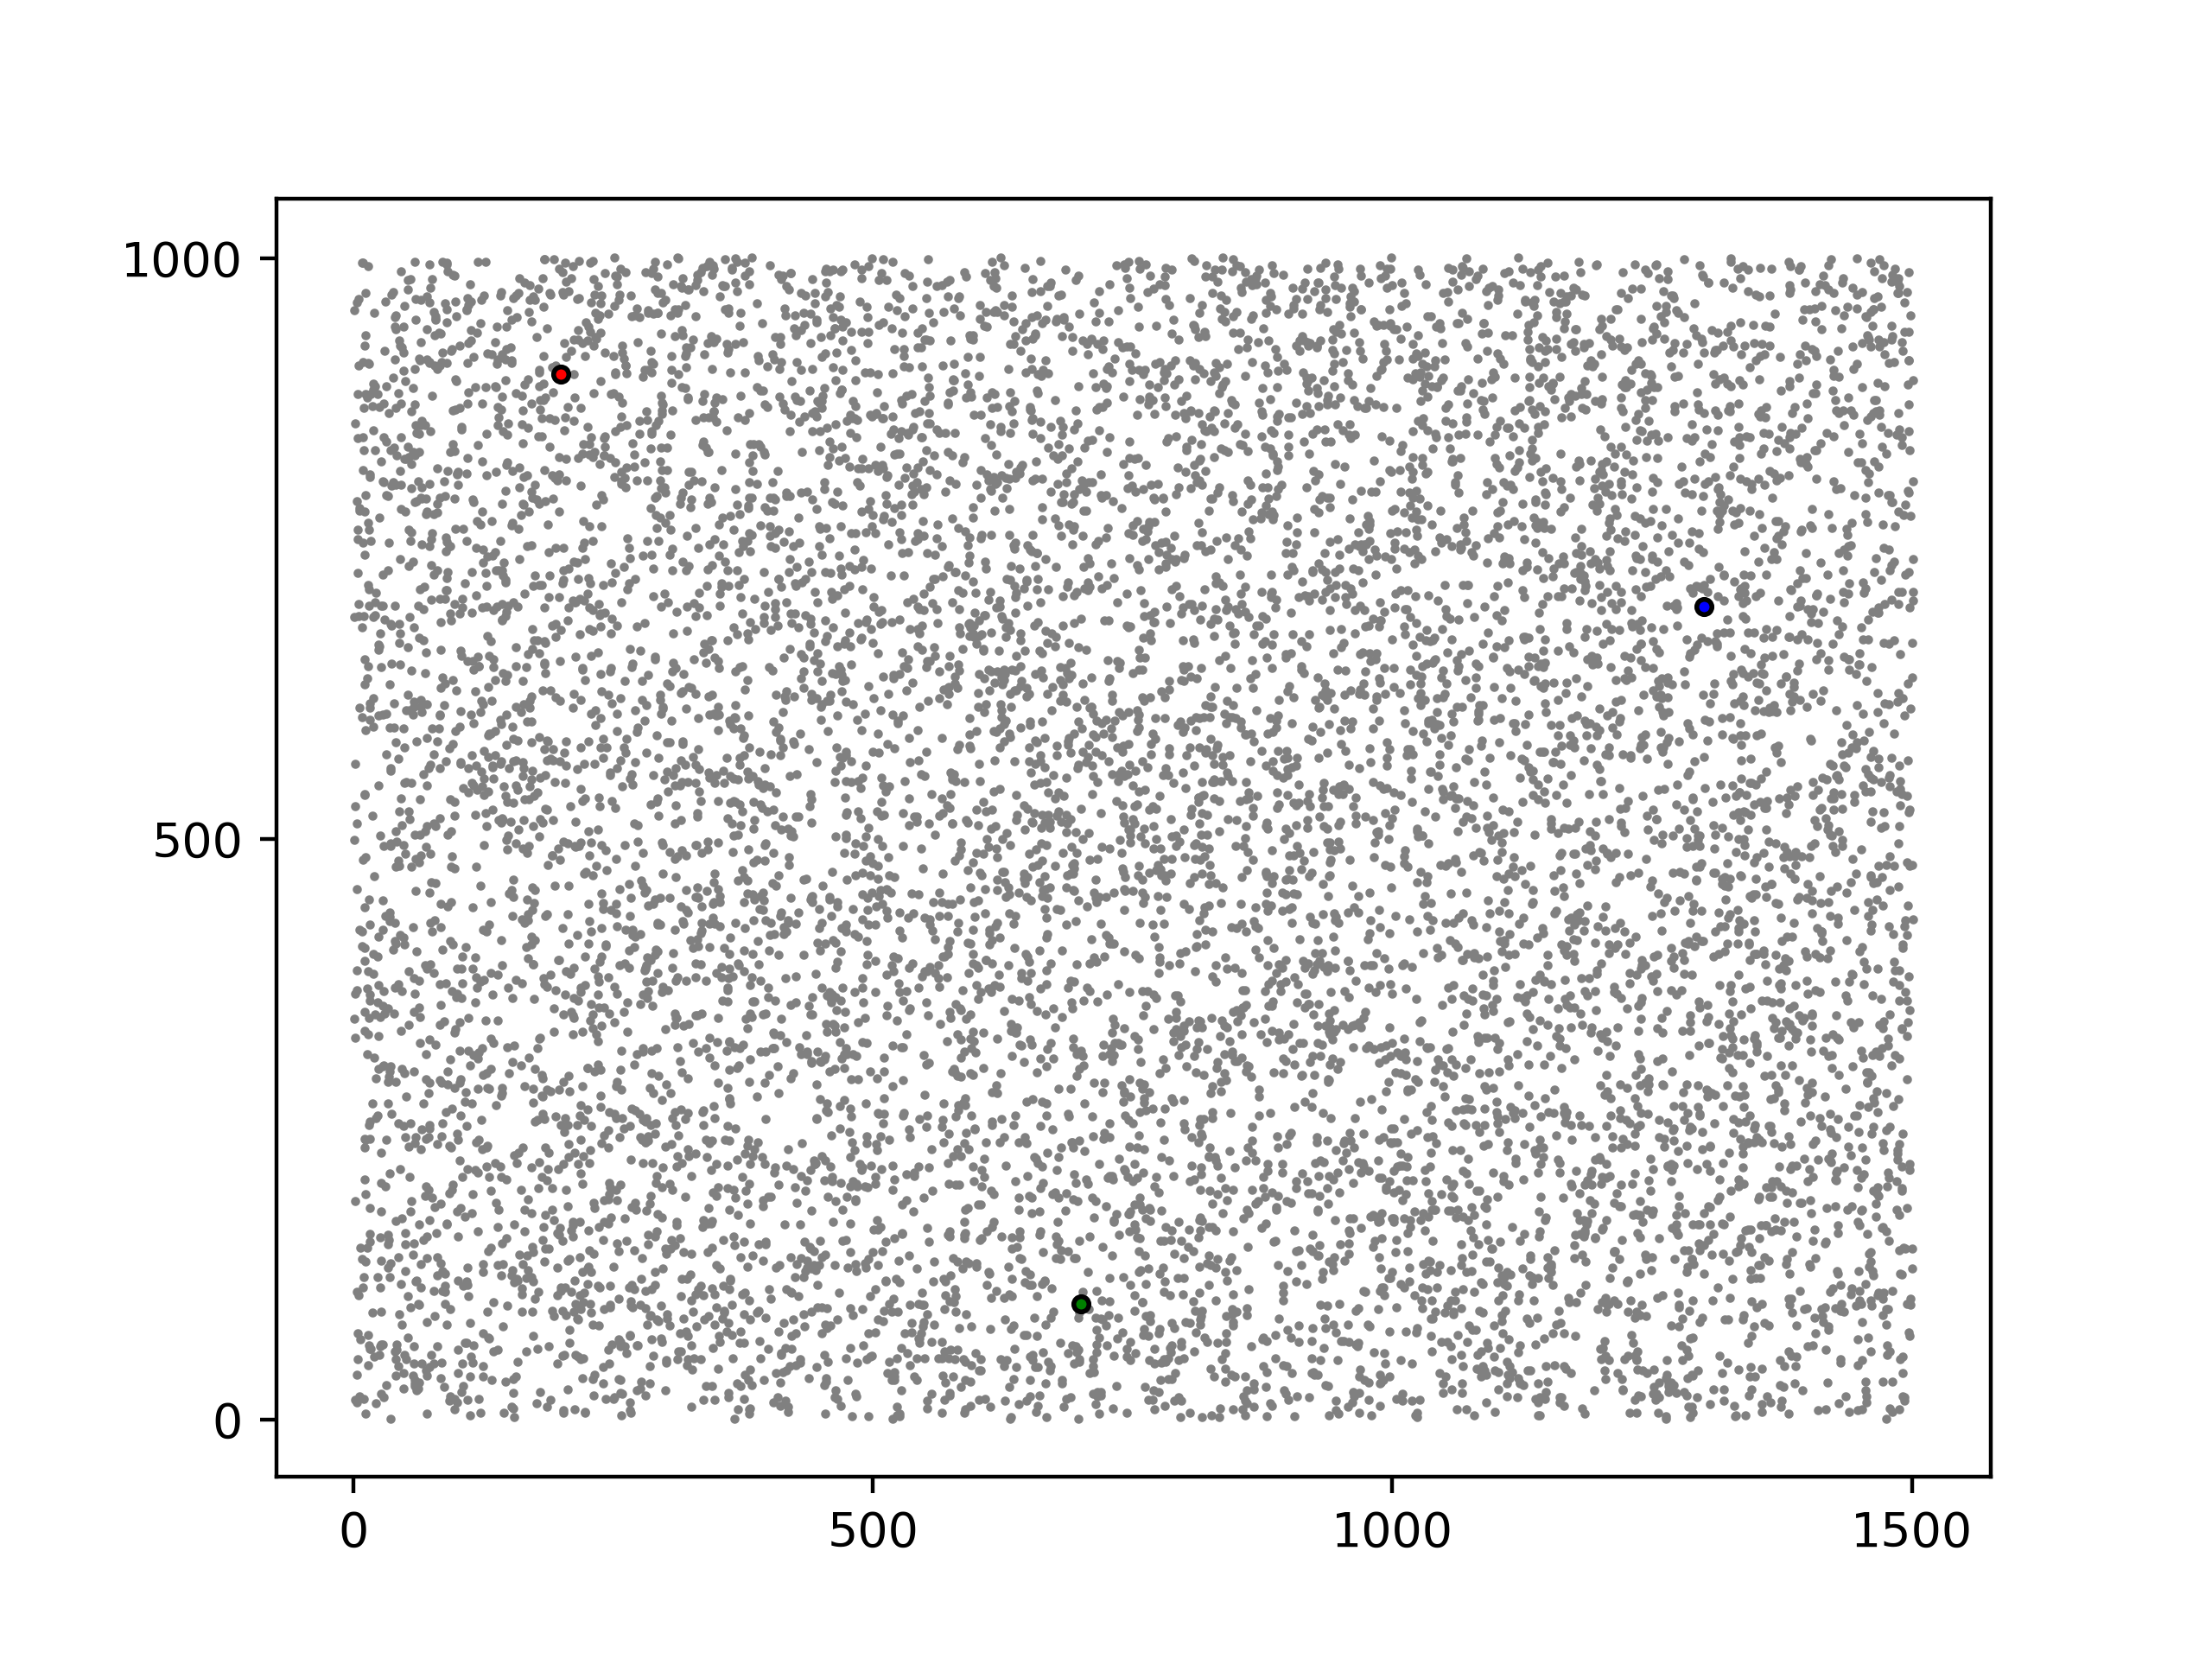
\includegraphics[width=\linewidth]{document/chapters/chapter_7/images/computation_start.png}
    \caption{Computation - Starting point}
    \label{fig:computation_start}
\end{figure}

\textbf{Given a Cartesian plane} (width: [0,1500], height: [0, 1000]) \textbf{and a set of 2D points} contained in it, \textbf{the map function takes as input one of said points and calculates the euclidean distance from each one of the centroids}; the centroid with \textbf{minimum distance among the three is then chosen, obtaining a key-value output} composed by the chosen class as the key and an array containing the computed point as the value (the array becomes relevant in the reduce function). It is important to note that, in comparing the distance among two points, the square root characterizing the euclidean distance is not needed and, therefore, it is not calculated in the map function.

\begin{lstlisting}[caption={Map function},captionpos=b]
const mapFunction = (p) => {
    const x = p[0];
    const y = p[1];
    const red = Math.pow(x - 200, 2) + Math.pow(y - 900, 2);
    const green = Math.pow(x - 700, 2) + Math.pow(y - 100, 2);
    const blue = Math.pow(x - 1300, 2) + Math.pow(y - 700, 2);
    switch(Math.min(red, green, blue)){
        case red: return ["red", [p]];
        case green: return ["green", [p]];
        case blue: return ["blue", [p]];
    }
}
\end{lstlisting}

Every data region is computed by the Map Workers and, \textbf{after every point in a particular region is classified, the output} (visualized in \textit{figure \ref{fig:computation_region_computation}}) \textbf{can be computed in the reduce function which simply reunites the intermediate results with the same key} (hence belonging to the same class) in a single array.

\begin{lstlisting}[caption={Reduce function},captionpos=b]
const reduceFunction = (p1, p2) => {
    p1.push(p2[0]);
    return p1;
}
\end{lstlisting}

\begin{figure}[!ht]
    \centering
    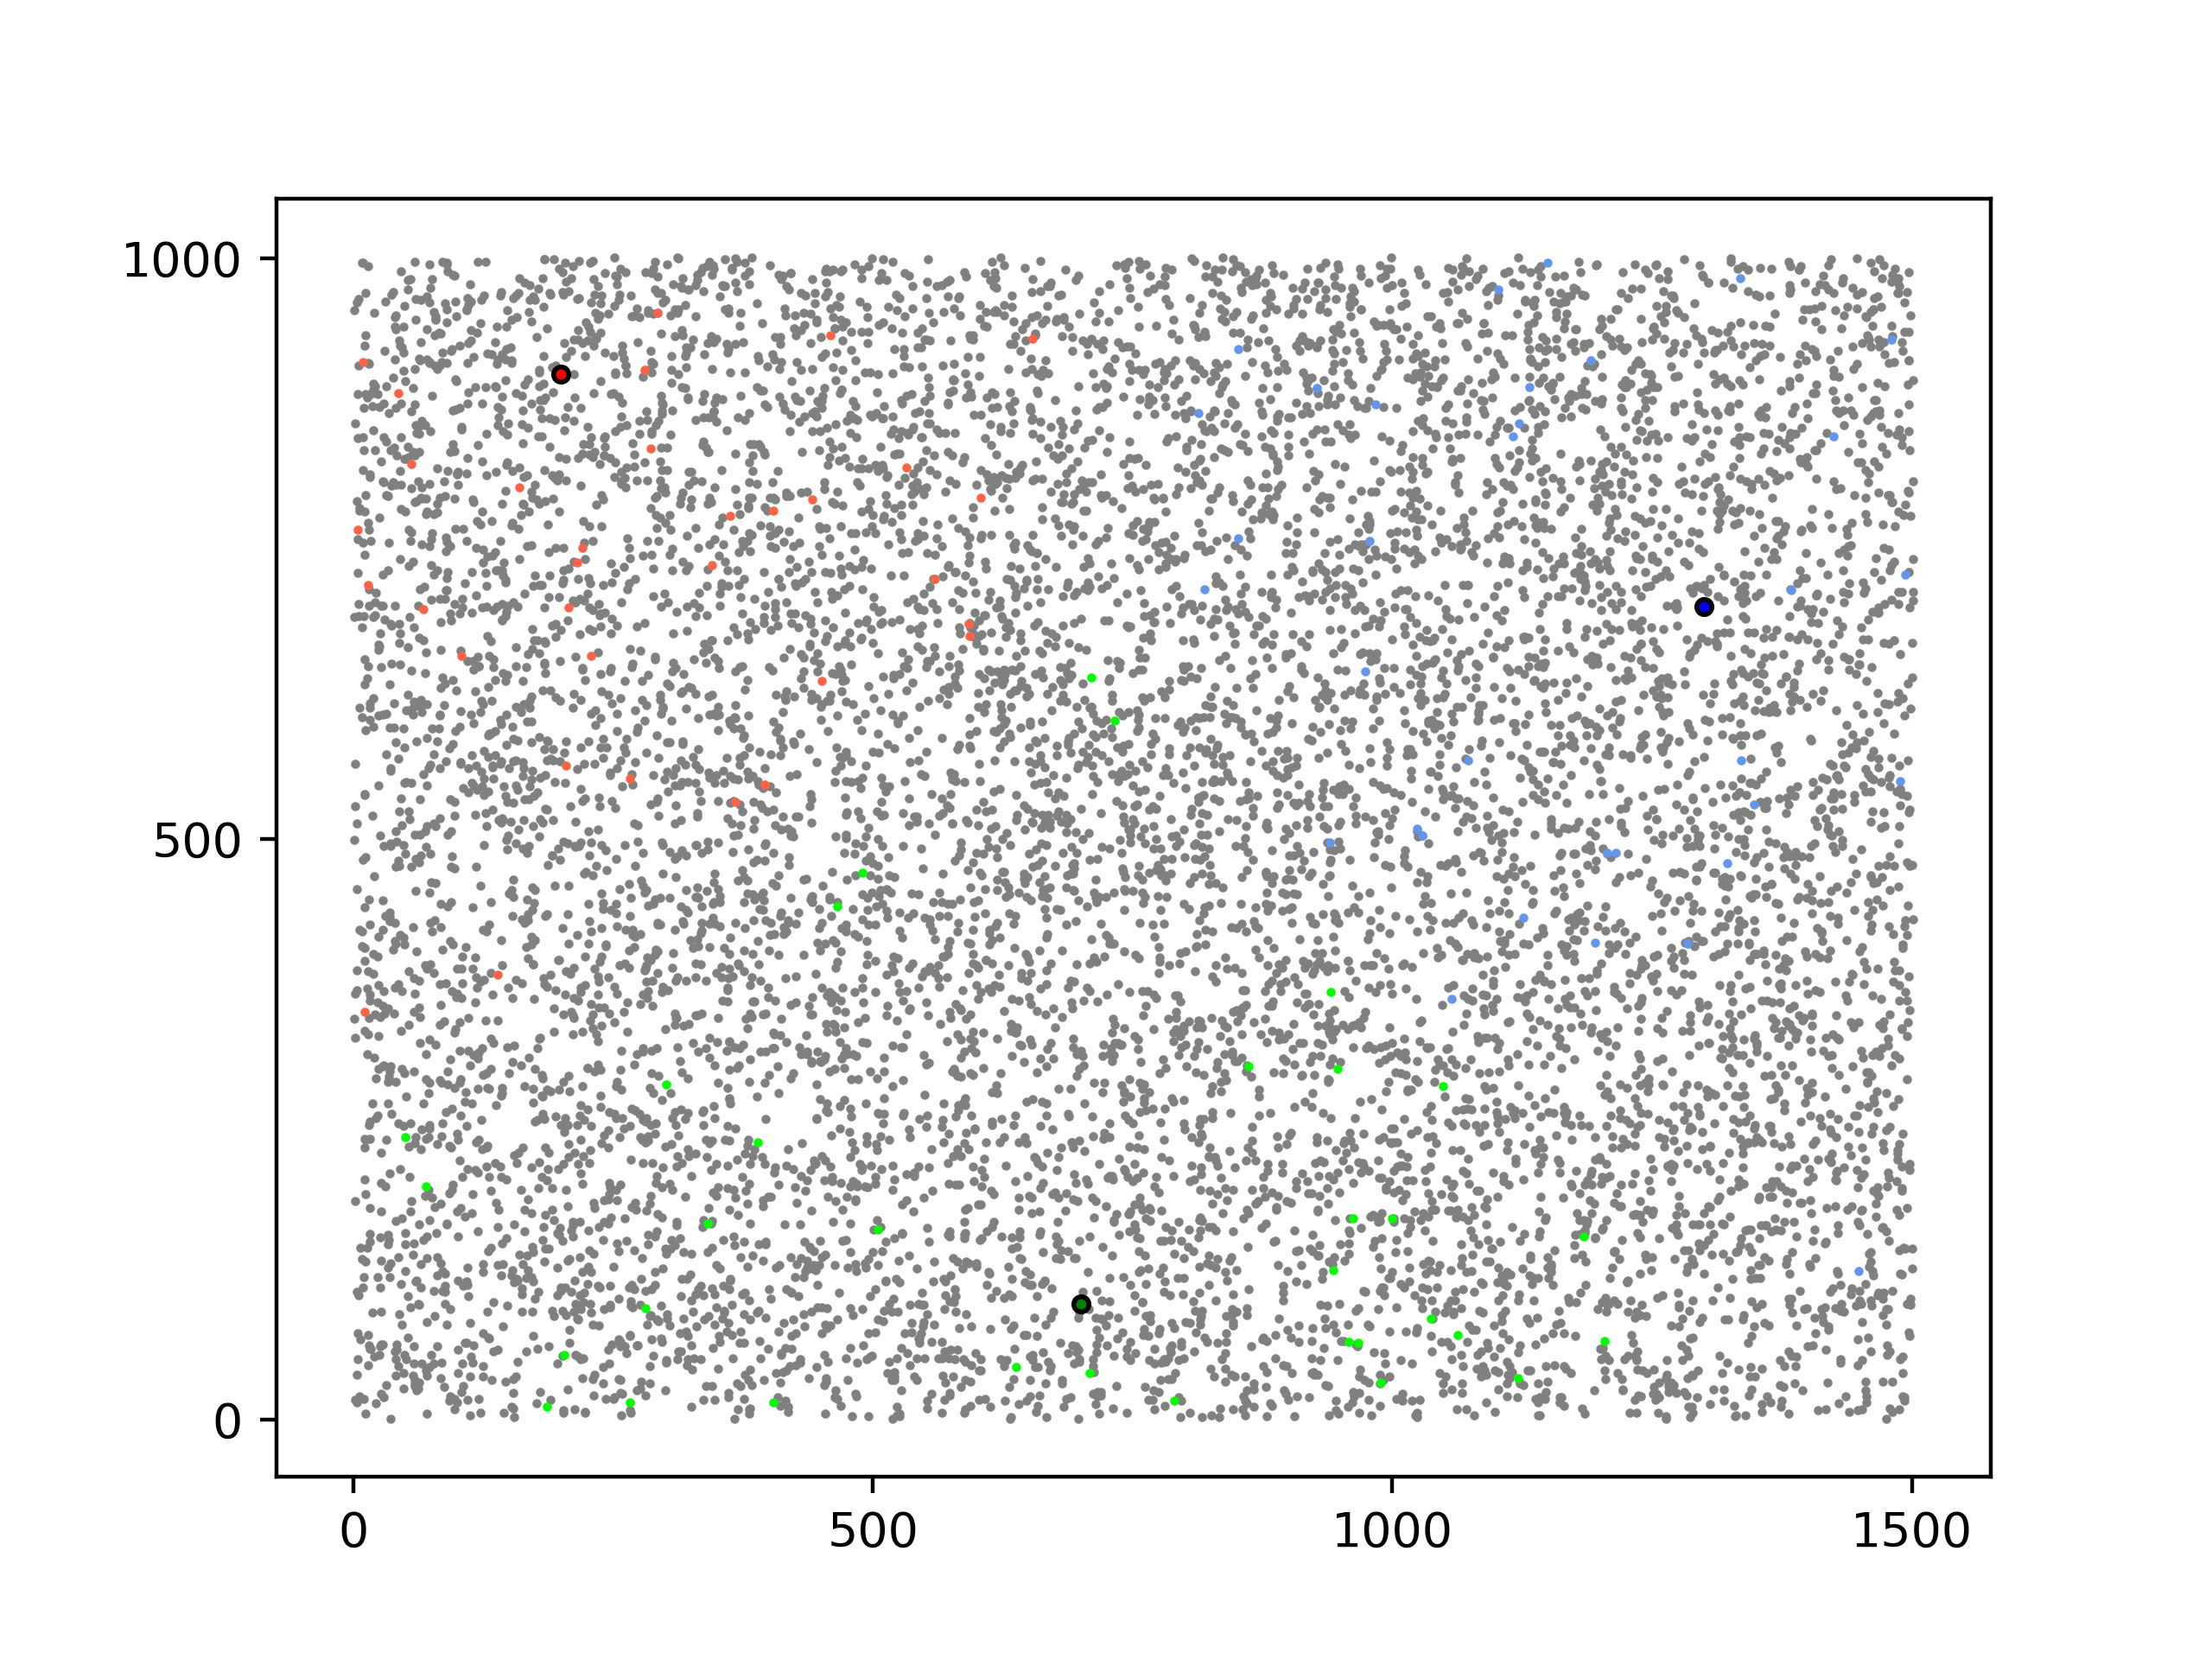
\includegraphics[width=\linewidth]{document/chapters/chapter_7/images/computation_region_computation.png}
    \caption{Computation - Region computation}
    \label{fig:computation_region_computation}
\end{figure}

As can be seen in \textit{figure \ref{fig:computation_final_result}}, after every region is mapped and then reduced, \textbf{each point is assigned to one of the three classes}.

\begin{figure}[!ht]
    \centering
    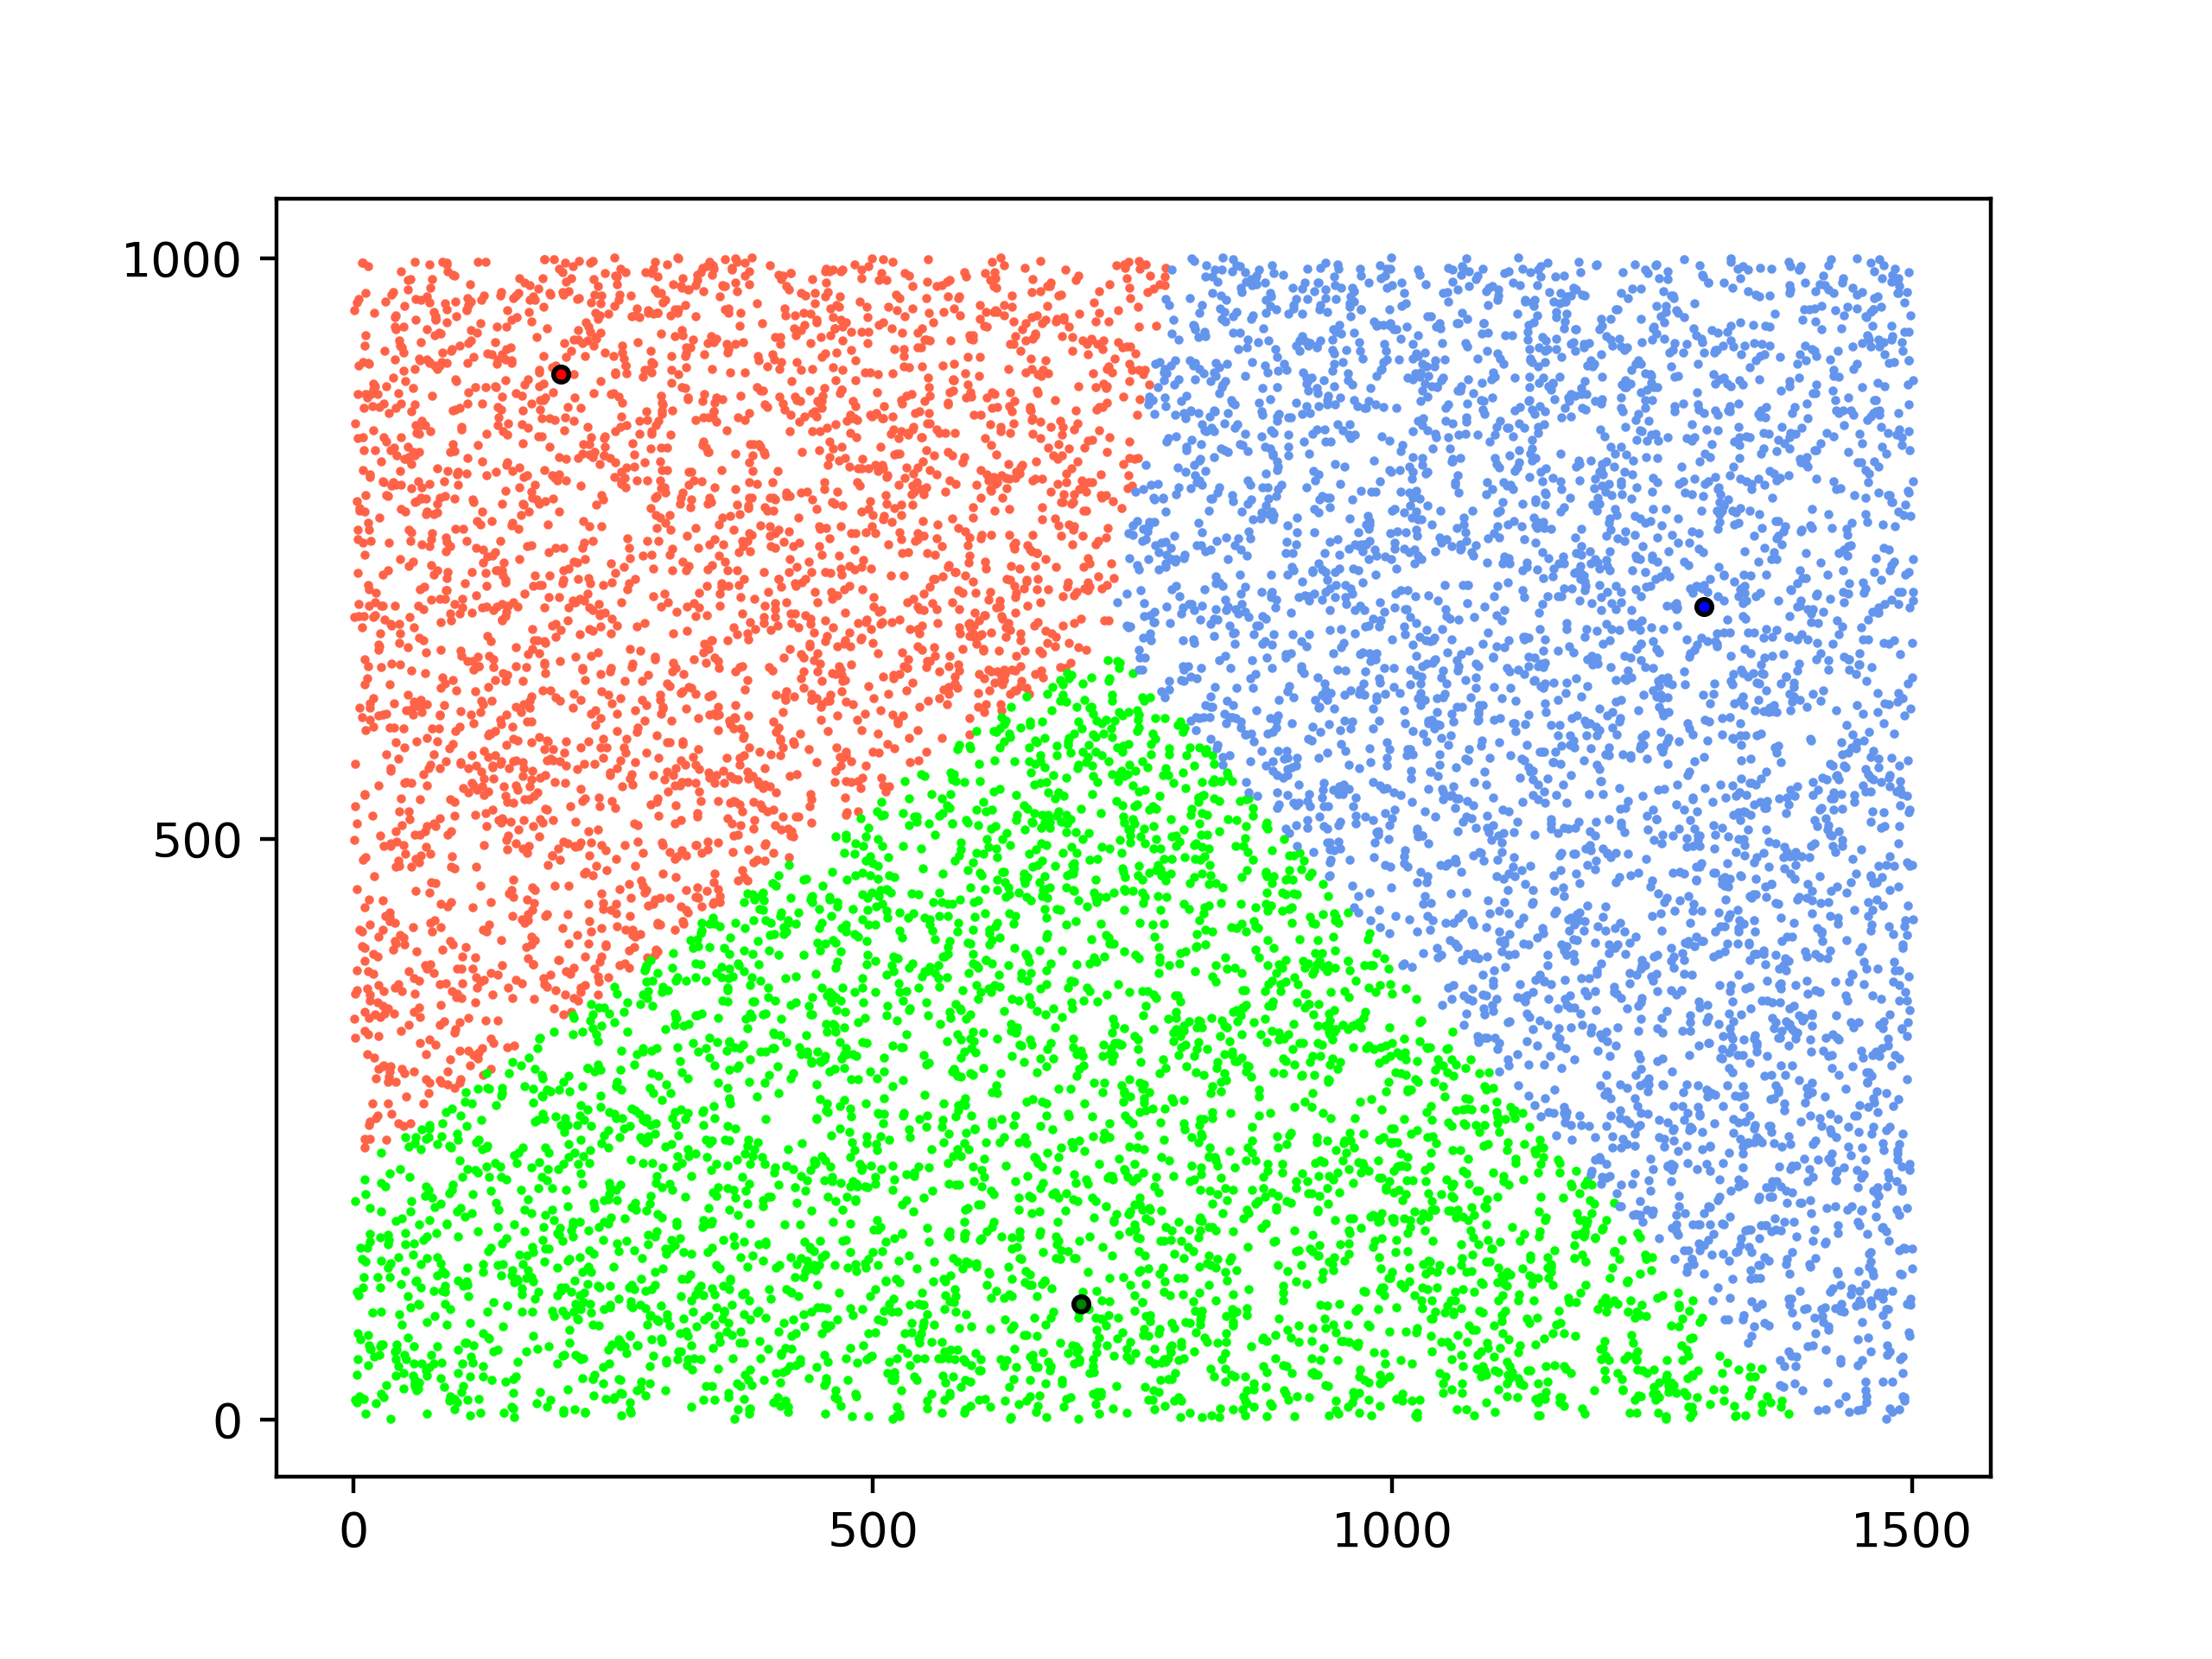
\includegraphics[width=\linewidth]{document/chapters/chapter_7/images/computation_final_result.png}
    \caption{Computation - Final result}
    \label{fig:computation_final_result}
\end{figure}

\textbf{Five experiments} were performed:
\begin{itemize}
    \item \textbf{1000 values} (10 regions, 100 points for each region)
    \item \textbf{10000 values} (100 regions, 100 points for each region)(shown in \textit{figure \ref{fig:computation_final_result}})
    \item \textbf{100000 values} (100 regions, 1000 points for each region)
    \item \textbf{1000000 values} (1000 regions, 1000 points for each region)
    \item \textbf{5000000 values} (2000 regions, 2500 points for reach region)
\end{itemize}

\subsection{Setup}
The experiment was performed in a controlled environment, meaning that only these devices were connected to the Grid (\textit{figure \ref{fig:experiment_devices_setup}}):
\begin{itemize}
    \item \textbf{A}: 1 smartphone
    \item \textbf{B}: 1 smartphone
    \item \textbf{C}: 1 computer
    \item \textbf{D}: 2 smartphones
    \item \textbf{E}: 1 tablet and 1 computer
\end{itemize}

\begin{figure}[!ht]
    \centering
    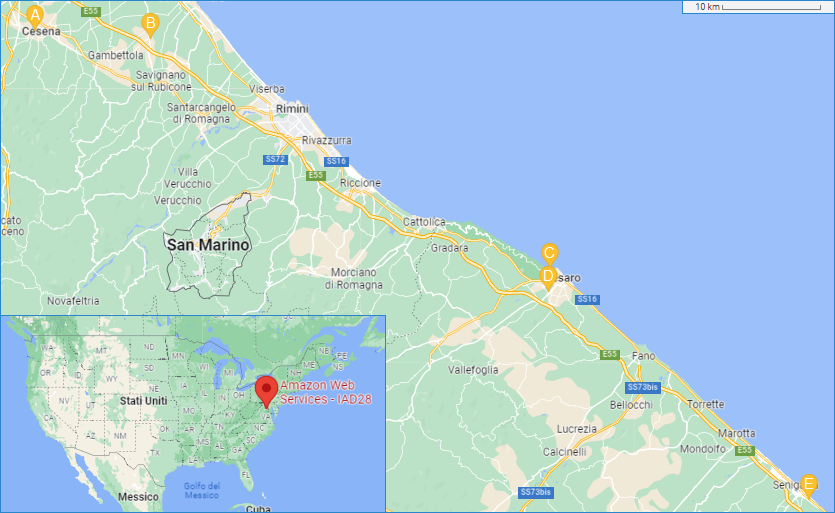
\includegraphics[width=\linewidth]{document/chapters/chapter_7/images/experiment_devices_setup.png}
    \caption{Devices setup}
    \label{fig:experiment_devices_setup}
\end{figure}

The setup of Contributing Endpoints was thus composed by \textbf{2 Interconnected Desktop Clients} and \textbf{5 Interconnected Mobile Clients}, placed in a \textbf{100 km range} in central Italy, which were forcibly chosen isolating them in a dedicated American server in order to perform multiple experiments with the same setup.

\textbf{The Invoking Endpoint Prototype instance was placed in the E location} (although it was not executed in the same computer which ran the Interconnected Desktop Client); said Invoking Endpoint requested the following resources for executing the MapReduce computation:
\begin{itemize}
    \item \textbf{4 Map Workers}
    \item \textbf{2 Reduce Workers}
\end{itemize}
    \textbf{Including the implicit MapReduce Master} (which will be taken by one of the two computers), \textbf{this adds up to the 7 devices specified earlier}, which were used in each of the five experiments.

\subsection{Results}
\textit{Figure \ref{fig:experiment_results}} shows the \textbf{results for the five experiments performed}, focusing on the \textbf{total time} and the \textbf{average time taken by each value} (both \textbf{measured in milliseconds}). Once again, these results were obtained using a very small pool of devices and the simplified nature of the MapReduce algorithm in this prototype significantly slows down the whole process (primarily because the intermediate results are first sent back to the MapReduce Master that then forwards them to the Reduce Worker, instead using a direct connection among Map Worker and Reduce Worker).

\begin{figure}[!ht]
    \centering
    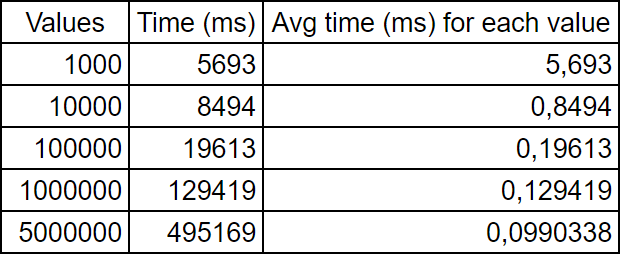
\includegraphics[scale=0.55]{document/chapters/chapter_7/images/experiment_results.png}
    \caption{Experiment results}
    \label{fig:experiment_results}
\end{figure}

The \textbf{first significant observation} can be made l\textbf{ooking at the first two experiments}: the \textbf{average time for each value drastically drops} (\texttildelow6.7 times faster); this can be \textbf{explained by considering that the total time also includes the recruitment phase where no computation is executed}. In other terms, \textbf{the number of values used in the first experiment is so small that their computation time becomes irrelevant}, meaning that the recruitment phase is basically the only factor that influences the average time. \textbf{The more values are computed (assuming the same number of devices are used), the less impactful the recruitment time becomes}.

\begin{figure}[!ht]
    \centering
    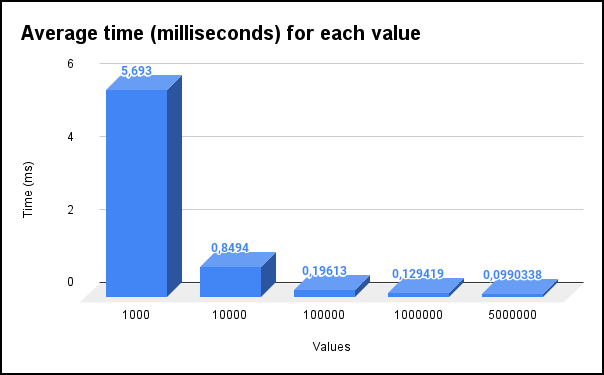
\includegraphics[scale=0.55]{document/chapters/chapter_7/images/experiment_results_avg_ms_per_value.png}
    \caption{Average time (milliseconds) for each value}
    \label{fig:experiment_results_avg_ms_per_value}
\end{figure}

Finally, \textit{figure \ref{fig:experiment_results_avg_ms_per_value}} focuses on \textbf{comparing the average time for each value}; it becomes apparent that, despite the not optimized algorithms used in this prototype, \textbf{the more values are computed, the greater the advantage becomes, showing that a distributed computation participated also by mobile devices is not only feasible, but it can also provide value to the Customer}.
